\documentclass{beamer}
\usepackage{amsmath}
%\usepackage{beamerthemesplit} % new 
\usetheme{Madrid}
\usefonttheme[onlymath]{serif}
\setbeamertemplate{frametitle}[default][center] %center slide titles

\begin{document}
\title{Notes on Siemens Ch. 3}
\author{Cody Petrie} 
\date{\today} 

%start slides
\frame{\titlepage} 

\frame{\frametitle{The Black Sphere}
\begin{itemize}
   \item Model neutron scattering from nuclei as a particle being absorbed by spherical object.
   \item Start by expanding an incident plane wave in terms of spherical harmonics.
   \begin{align}
      e^{i\mathbf{k}\cdot\mathbf{r}} &= \sum\limits_l C_l Y_l^0(\theta) \\
      e^{ikz} &\approx \sum\limits_l \frac{\sqrt{\pi}}{kr} \sqrt{2l+1} \, i^{l+1} \left( e^{-i(kr-\frac{l\pi}{2})} - e^{i(kr-\frac{l\pi}{2})} \right) Y_l^0(\theta)
   \end{align}
   \item Here we have used the fact that $\mathbf{k}\cdot\mathbf{r}$ only depends on $\theta$, and not on $\phi$, thus $m=0$. Also, we have used various identities and the orthonormality of spherical harmonics.
\end{itemize}
}

\frame{\frametitle{The Black Sphere}
\begin{itemize}
   \item Scattering only happens for short time
   \begin{equation}
      \phi(r\rightarrow\infty) = \sum\limits_l \frac{\sqrt{\pi}}{kr} \sqrt{2l+1} \, i^{l+1} \left( e^{-i(kr-\frac{l\pi}{2})} - \eta_l e^{i(kr-\frac{l\pi}{2})} \right) Y_l^0(\theta)
   \end{equation}
   \item Scattered wave is just the total wave function minus the incident wave function, $\phi_{sct} = e^{ikz}-\phi(r\rightarrow\infty)$.
   \begin{equation}
      \phi(r\rightarrow\infty) = e^{ikz} + f(\theta)\frac{e^{ikr}}{r}
   \end{equation}
   \begin{equation}
      f(\theta) = \sum\limits_l i \frac{\sqrt{\pi}}{k}\sqrt{2l+1} Y_l^0(\theta) (1-\eta_l)
   \end{equation}
   \item This looks like a scattering amplitude, $\frac{d\sigma}{d\Omega} = |f(\theta)|^2$.
\end{itemize}
}

\frame{\frametitle{The Black Sphere}
\begin{itemize}
   \item \textbf{Approximations:} Classical turning point is where $k^2 = l(l+1)/R^2 \approx (l+\frac{1}{2})^2/R^2$. If particle passes inside the range of force ($R$) you get absorption ($\eta_l = 0$), but if not you get none ($\eta_l$).
   \begin{equation}
      \frac{d\sigma}{d\Omega} = \frac{\pi}{k^2} \left|\sum\limits_{l=0}^{kr-1/2} \sqrt{2l+1} Y_l^0(\theta)\right|^2
   \end{equation}
   \item \textbf{More Approximations:} Here we approximate this for large and small angle scattering. I was not able to figure out the integrals so I'll just quote their answer here.
   \begin{align}
      \frac{d\sigma}{d\Omega} \approx
   \begin{cases}
      \frac{2R}{\pi} k\theta^2 \sin\theta\cos^2\left(kR\theta+\frac{\pi}{4}\right),& \text{for } kR\theta \gg 1 \\
      \frac{k^2R^4}{4}(1-(kR\theta/2)^2)^2,& \text{for } kR\theta \ll 1
   \end{cases}
   \end{align}
\end{itemize}
}

\frame{\frametitle{The Black Sphere}
\begin{figure}[h]
   \centering
   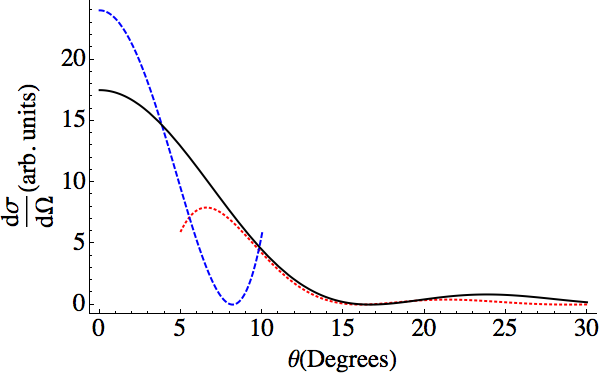
\includegraphics[width=0.4\textwidth]{../fig3_2.png}
   \caption{Rough reproduction of figure 3.2 in the book.}
\end{figure}
\begin{itemize}
   \item To find the angle of minumum scattering I have taken the derivative of the high angle scattering and set it equal to zero to get.
   \begin{equation}
      \theta_{min} = \frac{\pi}{4kR}(2n-1)
   \end{equation}
   \item Experiment must show that it's actually
   \begin{equation}
      \theta_{min} = \frac{5\pi}{4kR}
   \end{equation}
\end{itemize}
}

\frame{\frametitle{The Black Sphere}
\begin{equation}
   \theta_{min} = \frac{5\pi}{4kR}
\end{equation}
\begin{itemize}
   \item Now we can use this diffraction pattern to estimate the radius of nuclei. For Pb with $\epsilon = 84$ MeV we get $k = \sqrt{2m_N\epsilon/\hbar} \approx 2.0$ fm$^{-1}$. Now the graph above shows that $\theta_{min} \approx 15^\circ$. This gives us a radius of 7.5 fm.
   \item A quick google search gives Pb a radius of 7 fm.
\end{itemize}
}

\end{document}
